\chapter{SONUÇ}
Sayısal sinyal işleme algoritmaları, DSP ve GPGPU platformlarında koşturulmaktadır. Uygulamalar, karakteristik SIMD özellikleri sayesinde paralelleştirilerek hızlandırılmaya oldukça elverişli olduğu için son yıllarda GPGPU platformlarında CUDA ve OpenCL kullanılarak gerçeklenen sinyal işleme uygulamaları türetilmiştir. GPGPU mimarileri donanım seviyesinde özelleştirilemezken, platform bağımsız OpenCL sayesinde yüksek seviyede esnekliğe sahiptir. Öte yandan bazı uygulamalarda donanım seviyesinde değişiklikler yapmak istenebilir. Donanım seviyesinde değişiklik GPGPU donanımlarında mümkün olmadığı gibi ASIC tasarımlarda da maliyetlidir. Bu noktada FPGA tabanlı OpenCL destekli bir mimari hem donanım seviyesinde müdahale edilebilir, ölçeklenebilir bir yapıya hem de yazılım seviyesinde OpenCL'in sağladığı esnekliğe sahip olacaktır. Bu motivasyon ile tez çalışması dahilinde tasarlanan FPGA tabanlı yardımcı işlemci ünitesi tümüyle ölçeklenebilir ve özelleştirilebilir bir yapıya sahip olarak tasarlanmıştır.\par
\begin{itemize}
\item Belirlenen buyruk kümesi OpenCL kullanılarak yazılmış herhangi bir uygulamayı koşturabilecek kabiliyete sahiptir. 
\item Boru hattı mimarisi, aralıklı işlem modeli ve yazmaç öbeği, farklı warplardan buyrukların bir arada çalıştırılması ile veri bağımlılıkları çözülmeksizin boru hattının etkin kullanımını sağlamaktadır.
\item Tasarımın hiyerarşik olmasını sağlayan adalardan oluşan mimaride her ada içinde parametrik miktarda SIMD lane vardır. Bir adanın içindeki tüm SIMD lane'ler için aynı anda aynı buyruk çalıştırılırken farklı adalarda farklı buyruklar çalıştırılabilir. Bu sayede ortak kaynak kullanımı gerektiren ana bellek erişimi işlemlerine harcanan süre farklı adalar arasında faz farkı oluşturularak gizlenebilir.
\item Threadler arası veri paylaşımı paylaşımlı bellek üzerinden sağlanır. Her adada bir paylaşımlı bellek bulunmaktadır.
\item Paylaşımlı bellek farklı block ram'lere dağıtılmış bir adres uzayı üzerinde işlem yapmaktadır. Bu sayede SIMD lane adet port üzerinden gelen istekler çoğu durumda eş zamanlı olarak cevaplanabilmektedir. 
\item Paylaşımlı bellek adres uzayı, block ram'lere dağıttılırken ardışık adresler farklı block ramler'de olacak şekilde soyutlama yapılmıştır. Farklı portlardan gelen isteklerin eş zamanlı çalıştırılabilmesi için bu soyutlama ile yazılım seviyesinde optimizasyon imkanı sağlanmıştır. 
\item Hiyerarşik yapı, yazılım tarafından bakıldığında OpenCL destekli diğer platformlar gibi bazı kısıtlar getirmektedir. OpenCL ile gerçeklenmiş çekirdekler thread bloklarından oluşur. Her thread bloğunun içindeki threadler arasında veri paylaşımına izin vardır. Tosun mimarisinde her bir ada içinde paylaşımlı bellek gerçeklendiğinden bir adada çalışan herhangi bir thread, aynı ada içinde çalışan başka herhangi bir thread ile veri paylaşımında bulunabilir. Mevcut mimaride thread bloğu içindeki en fazla thread sayısı $N_{SIMD lane} x N_{warp}$ şeklinde ifade edilebilir. 
\item Hesaplama modüllerinin sabitlenmiş giriş çıkış ara yüzlerine uygun olmak şartı ile herhangi bir özel hesaplama modülü daha sonra tasarıma ilave edilebilir. Mevcut mimaride belirtilen buyruk kümesindeki tüm işlemler için gerekli olan hesaplama modülleri değişik sayılarda boru hattının hesap aşamasına eklenmiştir. Daha sonra ilave edilmek istenen bir hesap biriminden istenilen adette aynı giriş çıkış standardına bağlı kalınarak hesap aşamasına eklenebilir. Böylece buyruk kümesi genişletilebilir. 
\end{itemize}   

\section{Tosun Performans Analizi}
Tasarlanan mimaride performansın bir ölçütü buyrukların kaç çevrimde tamamlandığıdır. Her buyruğun boru hattını tamamlama süresi belli olsa da bir uygulamanın çalışmasında boru hattının etkin kullanımına göre toplam süre değişiklik gösterir. Mimariye uygun yazılan bir program için en iyi durumda boru hattı bir kere doldurulduktan sonra her çevrimde bir buyruk tamamlanır. Boru hattının uzunluğu hesap aşaması haricinde tüm buyruklar için sabittir. Hesap aşamasında ise her işlemin farklı bir süresi vardır. Her bir buyruk için hesap aşamasının tamamlanma süresi Tablo \ref{table:hesapSureleri}'de sunulmuştur. Tablo \ref{table:hesapSureleri}'de verilen "Hesaplama Ç.S.", matematiksel işlem için kullanılan zamandır. Hesap aşamasında hesaplama modülüne bağlı olarak giriş ve çıkışta kuyruk yapıları kullanılır. Boru hattının etkin kullanımı için eklenen bu kuyruklar, çevrim sayısında artışa sebep olur. Kuyrukların etkisiyle beraber, boru hattının hesaplama aşaması için her bir buyruğun toplam çevrim sayıları da "Boru Hattı Aşaması Ç.S." sütununda verilmiştir. \par

\begin{longtable}{p{50pt} p{90pt} p{90pt}}
\caption{Her Bir Buyruk için Hesap Aşaması Süreleri} \label{table:hesapSureleri} \\
\textbf{Buyruk} & \textbf{Hesaplama Ç.S.} & \textbf{Boru Hattı Aşaması Ç.S.}\\ 
\hline 
\endfirsthead

\multicolumn{2}{c}%
{{\bfseries \tablename\ \thetable{} -- devam}} \\
\textbf{Buyruk} & \textbf{Hesaplama Ç.S.} & \textbf{Boru Hattı Aşaması Ç.S.}\\ 
\hline 
\endhead

\hline \multicolumn{2}{r}{\textbf{Sonraki sayfada devam etmektedir.}} \\ 
\endfoot

\hline \hline
\endlastfoot
  addi		&  2 	&  4 \\
  andi 		&  0  &  2 \\
  ori 		&  0  &  2 \\
  xori 		&  0  &  2 \\
  divi 		&  20 & 24 \\
  muli 		&  2  &  4 \\
  subi 		&  2  &  4 \\
  movi 		&  0  &  2 \\
  movhi		&  0  &  2 \\
  fabs  	&  0  &  2 \\
  fadd  	&  5  &  7 \\
  fcom  	&  1  &  3 \\
  fdiv  	&  10 & 14 \\
  fmul  	&  2  &  4 \\
  fsqrt  	&  14 & 18 \\
  fcos  	&  28 & 32 \\
  fsin  	&  28 & 32 \\
  ffma  	&  9  & 11 \\
  ffms  	&  9  & 11 \\
  fmin  	&  0  &  2 \\
  fmax  	&  0  &  2 \\
  fln 	 	&	 12 & 16 \\
  fmod 		&	 10 & 14 \\
  f2int 	&	    &  4 \\
  int2f		&	    &  4 \\
  fchs		&	  0 &  2 \\
  fexp 		&	  8 & 12 \\
  add 		&	  2 &  4 \\
  and 		&	  0 &  2 \\
  or 		  &	  0 &  2 \\
  xor		  &	  0 &  2 \\
  div  		&  20 & 24 \\
  mul  		&   2 &  4 \\
  shl  		&   1 &  3 \\
  shr  		&   1 &  3 \\
  shra  	&   1 &  3 \\
  sub  		&   2 &  4 \\
  min  		&   1 &  3 \\
  max  		&   1 &  3 \\
  chs  		&   2 &  4 \\
  not  		&   0 &  2 \\
  abs  		&   2 &  4 \\
  com  		&   1 &  3 \\
  mod  		&   2 & 24 \\
  brv 		&	  0 &  2 \\
  bfr 		&	  1 &  3 \\
  br 			&	  x &  x \\
  fin 		&	  x &  x \\
  ldshr 	&	 7-22 & 1 - 26 \\
  stshr 	&	 7-22 & 1 - 26 \\
  sync		&	  x  & x \\
  ldram 	&	   &  \\
  stram		&	   &  \\
  mov 		&    0 & 2 \\
  jmp  		&    x & x \\
  
\end{longtable}

Tosun üzerinde çalıştırılan bir buyruk işlenmek üzere bir adaya alındıktan sonra tüm boru hattı aşamalarından geçerek işlemini tamamlar. Tablo \ref{table:hesapSureleri}'de sunulan boru hattı aşaması çevrim sayıları yalnızca hesaplama aşamasına ait verilerdir. Nitekim buyruklar arası çevrim sayısı farklılıkları yalnızca hesaplama aşamasında oluşmaktadır. Diğer tüm boru hattı aşamaları, tüm buyruklar için sabit çevrim sayısına sahiptir.\par

Tasarlanan boru hattında bir buyruğun çalışması warp seçimi ile başlar. Warp seçimi donanımda aktif warp'ların tutulduğu bir tablo üzerinde Round Robin algoritması ile seçim yapılmasından ibarettir ve 1 çevrimde sonuçlanır. \par 

Seçilen warp için sıradaki buyruk bellekten çekilir. Bu aşamada buyruk ön belleğinde söz konusu buyruk bulunursa, 1 çevrimde aşama geçilir. Eğer buyruk önbellekte yoksa, ana bellek üzerinden buyruğun çekilmesi gerekmektedir. Ana belleğin cevap süresi anlık yoğunluğa göre değişmektedir. En kötü durum, tüm adaların hem veri hem buyruk portlarından istek gelirken aynı zamanda PCI ve ana bellek arasında da veri akışı varken, hiçbir isteğin önbellekte bulunamaması durumudur. En kötü durum tahmini cevap süresi $35 x ( N_{ada} x 2 + 1 )$ şeklinde ifade edilebilir. Buyrukların ana bellekten çekilmesi bloklar halinde yapılır. Tek seferde 512 bit yani 16 adet buyruk çekilir. Dolayısıyla en kötü durum gerçekleştiğinde yaşanan gecikme, her 16 buyruk için bir kez yaşanır. Burada dallanma buyruğu gelmesinden dolayı yanlış buyrukların çekilmiş olması senaryosu daha kötü bir durum olarak düşünülür fakat Tosun işlemcisinde her SIMD lane üzerinde koşan thread dallanma neticesinde farklı davranabileceğinden ve SIMD mimarisinin uygulanmasından dolayı dallanmalarda her iki ihtimal de her SIMD lane üzerinde sonuçlar maskelenerek çalıştırıldığından dallanma oluşması buyruk çekme açısından ek bir maliyete sebep olmaz.\par

\begin{figure}[ht] \label{image:fillPipelineBestWorst}
\centering
\shorthandoff{=}
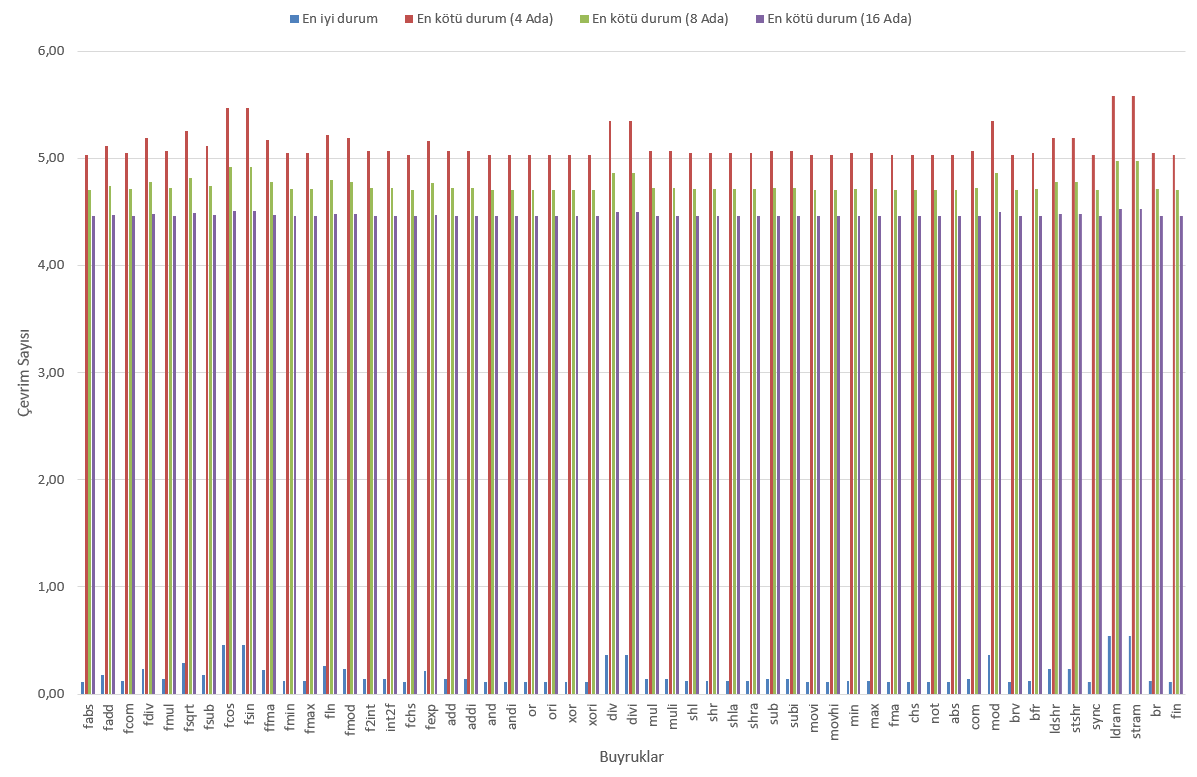
\includegraphics[width=0.9\textwidth]{gorsel/fillPipelineBestWorst.png}
\shorthandoff{=}
\caption{En iyi ve en kötü durumlarda buyruk başına çevrim sayısı}
\end{figure}

Buyruk çözme aşamasında yalnızca bit gruplarının ayrılması işlemi yapıldığından 1 çevrimde geçilebilir. Yazmaç çekme aşamasında her SIMD lane kendine ait yazmaç öbeğinden 1, 2 veya 3 adet yazmacın değerini okur. Yazmaç öbeğinin cevap süresi en kötü durumda 3, ortalamada 1 çevrimdir.\par
Hesap modülü atama aşamasında işlem koduna göre hesaplama birimlerinden biri hesaplamayı yapmak üzere seçilir ve gerekli giriş değerleri iletilir. Basit karşılaştırma devrelerinden oluşan aşama 1 çevrimde tamamlanır. Hesaplama aşaması ise her buyruk için farklı cevap süresine sahiptir. \par
Hesaplamanın bitmesi ile birlikte hesaplama modüllerinin çıkışında bulunan tampon belleklerde sonuçlar yazılmak üzere sıraya alınır. Geri yazma gerektirmeyen veya yanlış bir dallanma ile gelen buyruklar bu aşamada yazılmaz fakat işlem süresi olarak beklemek zorundadırlar. Geri yazma işlemi sonucu yazmaç öbeğine yazarken warp listesinde de buyruğun ait olduğu warp'un hazır bayrağını 1 yapar. Böylece aynı warp daha sonra tekrar seçilebilir. Geri yazma aşaması toplamda 1 çevrimde tamamlanır.\par

Sonuç olarak herhangi bir buyruğun boru hattını baştan sona tamamlaması için gerekli çevrim sayısı en kötü durum için Denklem \ref{equation:pipelineCycleEstimationWorstCase}'de belirtildiği şekilde, en iyi durum için Denklem \ref{equation:pipelineCycleEstimationBestCase}'de belirtildiği şekilde hesaplanabilir.\par

\begin{align} \label{equation:pipelineCycleEstimationWorstCase}
	T_{boru hatti} 	&= 1 + 35x(2N_{ada} + 1) + 1 + 3 + 1 + T_{hesap} + 1 \\
									&= T_{hesap} + 35 x (2N_{ada}+1) + 7
\end{align}

\begin{align} \label{equation:pipelineCycleEstimationBestCase}
	T_{boru hattı}  &= 1 + 2 + 1 + 3 + 1 + T_{hesap} + 1 \\
									&= T_{hesap} + 9
\end{align}

Her buyruk için en iyi durum ve en kötü durumda çevrim sayısı, 16 SIMD lane'den oluşan 4 ada için Şekil \ref{image:fillPipelineBestWorst}'de sunulmuştur. Grafikte gösterilen çevrim sayıları, en kötü durumda buyruk başına boru hattının dolması için geçen süreyi ifade etmektedir. Boru hattının doldurulmasından sonra her çevrimde bir sonuç verilmesi beklendiğinden Şekil \ref{image:fillPipelineBestWorst}'de sunulan değerler olabilecek en kötü sonuçlardır.\par



Mimaride ada sayısının artışı ile aynı anda çalışabilecek thread bloklarının sayısı, dolayısıyla paralellik artmaktadır. Öte yandan ana bellek veri yolu genişliği sabit olup paralelleştirmede kısıtlayıcı etkendir. Mimaride eş zamanlı koşturulan toplam thread sayısının artırılması bellek işlemlerinde gecikmeyi artırır. En kötü durumda buyruk başına boru hattının ortalama dolma sürelerinin ada sayısına göre değişimi Şekil \ref{image:fillPipelineWorstVsNumOfIslands}'de sunulmuştur.\par

\begin{figure}[ht]
\centering
\shorthandoff{=}
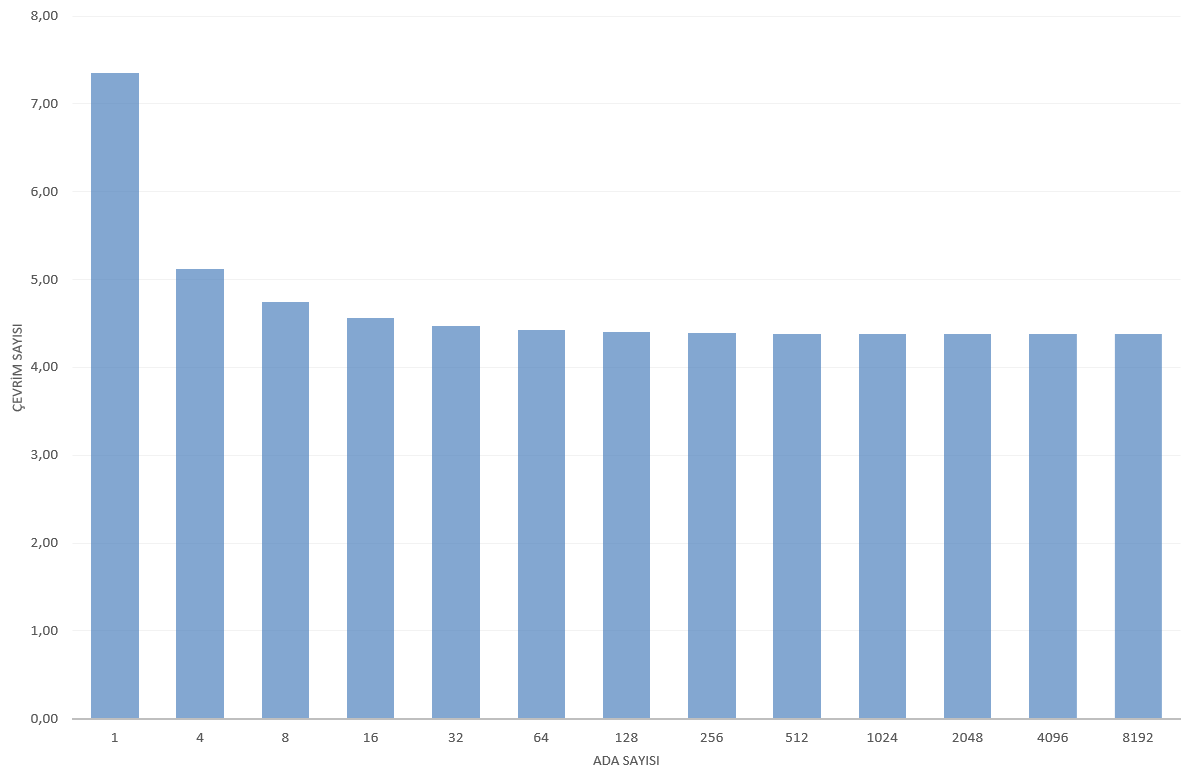
\includegraphics[width=0.9\textwidth]{gorsel/fillPipelineWorstVsNumOfIslands.png}
\shorthandoff{=}
\caption{Ortalama buyruk başına çevrimin ada sayısına göre değişimi}
\label{image:fillPipelineWorstVsNumOfIslands}
\end{figure}

Yukarıda da belirtildiği gibi sunulan değerler boru hattının doldurulması ile ilgili değerlerdir. N adet buytruktan oluşan bir programın ortalama çalışma süresi Denklem \ref{}'de sunulduğu şekilde hesaplanır. \par

\begin{align} \label{equation:pipelineCycleEstimationWorstCase}
	T_{program}= T_{hesap} + 7 + (N_{buyruk}/16) x 35 x N_{ada}
\end{align}

$T_{hesap}$ tüm buyrukların hesağlanması için geçen süreyi ifade eder ve programın içerdiği buyruk tiplerine ve sayılarına bağlı olarak değişir. Örneğin standart bir FFT uygulaması için yazılan bir programın boru hattı üzerinde ilerleyişi incelenerek toplam çalışma süresi hesaplanmıştır. Karşılaştırma amaçlı olarak Xilinx tarafından sağlanan FFT IPCore'unun tahmini çalışma süreleri alınmıştır. Değişik örnek sayıları için çalışma süreleri 250 MHz sıklığında saat çevrimi sayısı cinsinden Tablo \ref{table:fftComparision}'de sunulmuştur.

\begin{longtable}{p{90pt} p{90pt} p{120pt}}
\caption{} \label{table:fftComparision} \\
\textbf{Nokta Sayısı} & \textbf{Tosun Ç.S.} & \textbf{Xilinx IPCore Ç.S.}\\ 
\hline 
\endfirsthead

\multicolumn{2}{c}%
{{\bfseries \tablename\ \thetable{} -- devam}} \\
\textbf{Nokta Sayısı} & \textbf{Tosun Ç.S.} & \textbf{Xilinx IPCore Ç.S.}\\ 
\hline 
\endhead

\hline \multicolumn{3}{r}{\textbf{Sonraki sayfada devam etmektedir.}} \\ 
\endfoot

\hline \hline
\endlastfoot
8		& 242		& 80 \\
16		& 321		& 160 \\
32		& 400		& 320 \\
64		& 479		& 640 \\
128		& 558		& 1280 \\
256		& 1190		& 2560 \\
512		& 2612		& 5120 \\
1024	& 5772		& 10240 \\
2048	& 12724		& 20480 \\
4096	& 27892		& 40960 \\
8192	& 60756		& 81920 \\
16384	& 131540	& 163840 \\
32768	& 283220	& 327680 \\
65536	& 606804	& 655360 \\
\end{longtable}

Tablo \ref{table:fftComparision}'de gözlendiği şekilde sinyalde nokta sayısının artması ile Tosun mimarisi, IPCore'a göre daha yüksek performans göstermektedir. Bunun sebebi nokta sayısının artması ile paralelleştirmenin avantajının artmasıdır. Karşılaştırmanın herhangi bir GPU, CPU veya ASIC tabanlı uygulama yerine IPCore ile karşılaştırılmasının sebebi IPCore'un Tosun mimarisi ile aynı FPGA platformunda çalıştırılabilmesidir. Diğer platformlarla karşılaştırmak için çevrim sayıları $4x10^{-9}$ ile çarpılarak saniye cinsinden zaman değerlerine ulaşılabilir. \par

\section{Tosun Kaynak Kullanımı Analizi}
Tosun mimarisinin büyük kısmını oluşturan ada yapısı alt modülleri seviyesinde irdelenerek devrenin alan değerlerine karşın performansındaki değişim gözlenmiştir. Hedef platform olarak belirlenen Virtex7 FPGA'in kapasitesi Tablo \ref{table:virtex7Resources}'de verilmiştir.

\begin{longtable}{p{90pt} p{90pt}}
\caption{Virtex 7 VC709 Geliştirme Kartı Kaynak Kapasitesi} \label{table:virtex7Resources} \\
\textbf{Kaynak} & \textbf{Kapasite}\\ 
\hline 
\endfirsthead

\multicolumn{2}{c}%
{{\bfseries \tablename\ \thetable{} -- devam}} \\
\textbf{Kaynak} & \textbf{Kapasite}\\  
\hline 
\endhead

\hline \multicolumn{2}{r}{\textbf{Sonraki sayfada devam etmektedir.}} \\ 
\endfoot

\hline \hline
\endlastfoot
Slice LUT & 433200 \\
Slice Register & 866400\\
Block RAM & 2940 RAMB18\\
DSPs & 3600\\
I/O & 1032\\
\end{longtable}

Adanın her bir alt parçası hedef platforma göre sentezlenerek kaynak kullanımları gözlenmiştir. Hesap modüllerinin sayılarında değişikliğe gidilerek farklı kombinasyonlarda kaynak kullanımı gözlenmiş ve performansa etkisi irdelenmiştir.\par
\begin{figure}[ht]
\centering
\shorthandoff{=}
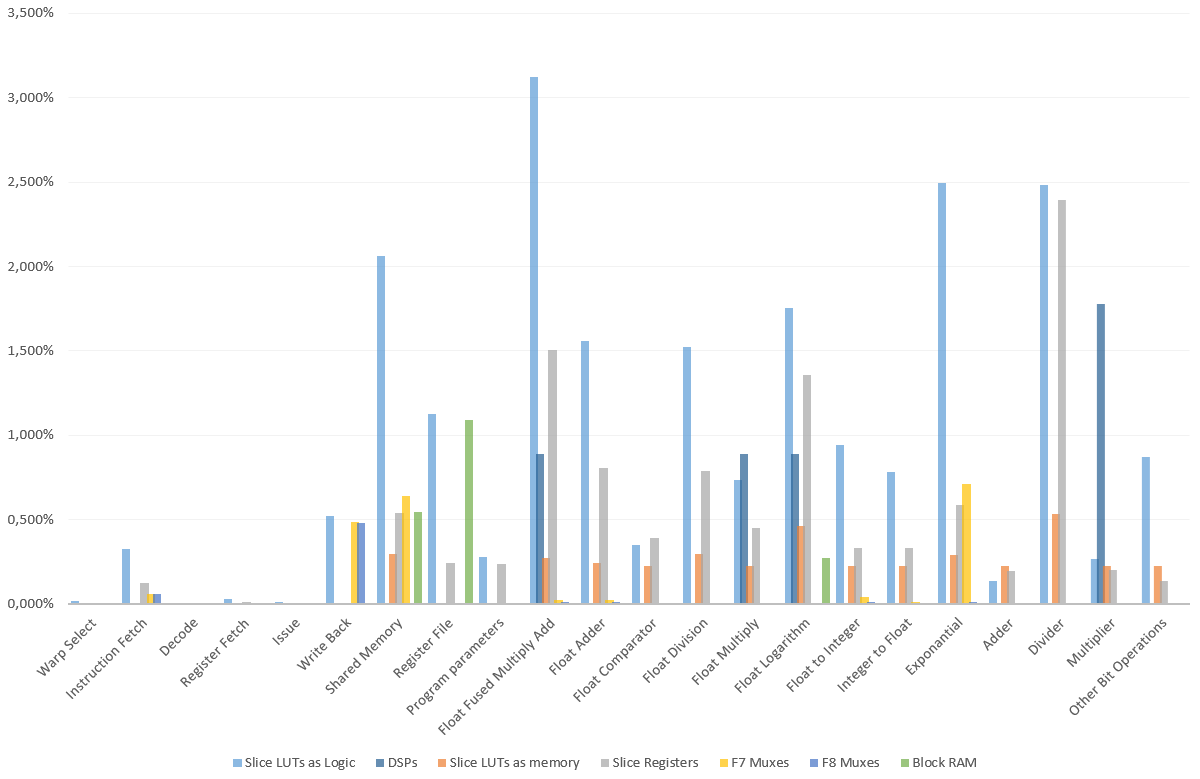
\includegraphics[width=0.9\textwidth]{gorsel/Util_S16_FMA16_O8.png}
\shorthandoff{=}
\caption{Ada alt modüllerinin kaynak kullanımı (Konfigurasyon 1)}
\label{image:util_S16_FMA16_O8}
\end{figure}
Şekil \ref{image:util_S16_FMA16_O8}'de 16 SIMD lane'e sahip bir adada tüm hesap birimlerinden 16, float bölme, logaritma, üssel fonksiyon ve tamsayı bölme birimlerinden 8 adet gerçeklenmiştir. Elde edilen kaynak tüketim değerlerine göre 1 ada hedef platformun kaynaklarının \%21.4'ünü kullanmaktadır. Dolayısıyla platformda en fazla 4 adet adadan söz edilebilir. Her bir adada 16 SIMD lane ve 32 warp bulunduğundan eş zamanlı olarak platform üzerinde çalışabilecek toplam thread sayısı 2048'dir. Bu seçenekte adalar yerleştirildikten sonra boş kalan \%14'lük kısım bellek ara yüzü, PCI-e arayüzü ve scheduler için değerlendirilir. Bu konfigurasyon için float bölme, logaritma, üssel fonksiyon ve tamsayı bölme işlemlerinde fazladan 1 çevrim hesap süresi, fazladan 2 çevrim kuyruklama süresi eklenir. Değişiklik ile 16 adet sayının hesaplanması için harcanan süredeki değişim Tablo\ref{table:util_S16_FMA16_O8}'de sunulmuştur. Buradaki değişiklik, boru hattının dolması sırasında söz konusudur. Boru hattı doldurulduktan sonra "throughput" olarak her çevrimde 1 sonuç alınır.\par 

Şekil \ref{image:util_S16_FMAFDIVFLOG8_FEXPDIV4}'de 16 SIMD lane'e sahip bir adada tüm hesap birimlerinden 16, float çarp topla, float bölme ve logaritma 8'er adet, üssel fonksiyon ve tamsayı bölme birimlerinden 4'er adet gerçeklenmiştir. Elde edilen kaynak tüketim değerlerine göre 1 ada hedef platformun kaynaklarının \%17.37'sini kullanmaktadır. Dolayısıyla platformda en fazla 4 adet adadan söz edilebilir.\par
\begin{longtable}{p{90pt} p{90pt} p{90pt} p{90pt}}
\caption{Bölme, logaritma ve üssel fonksiyon hesaplama birimlerinin yarıya düşürülmesinin performansa etkisi} \label{table:util_S16_FMA16_O8} \\
\textbf{İşlem} & \textbf{Eski Hesap Süresi} & \textbf{Yeni Hesap Süresi} & \textbf{Yüzde Değişim} \\ 
\hline 
\endfirsthead

\multicolumn{2}{c}%
{{\bfseries \tablename\ \thetable{} -- devam}} \\
\textbf{İşlem} & \textbf{Eski Hesap \newline Süresi} & \textbf{Yeni Hesap \newline Süresi} & \textbf{Yüzde Değişim} \\ 
\hline 
\endhead

\hline \multicolumn{2}{r}{\textbf{Sonraki sayfada devam etmektedir.}} \\ 
\endfoot

\hline \hline
\endlastfoot
Float Bölme & 12 & 15 & \%25\\
Logaritma & 14 & 17 & \%21\\
Üssel & 10 & 13 & \%30\\
Tam Sayı Bölme & 22 & 25 & \%14\\
\end{longtable}
Her bir adada 16 SIMD lane ve 32 warp bulunduğundan eş zamanlı olarak platform üzerinde çalışabilecek toplam thread sayısı 2048'dir. Bu seçenekte adalar yerleştirildikten sonra boş kalan \%14'lük kısım bellek ara yüzü, PCI-e arayüzü ve scheduler için değerlendirilir.\par

\begin{figure}[ht]
\centering
\shorthandoff{=}
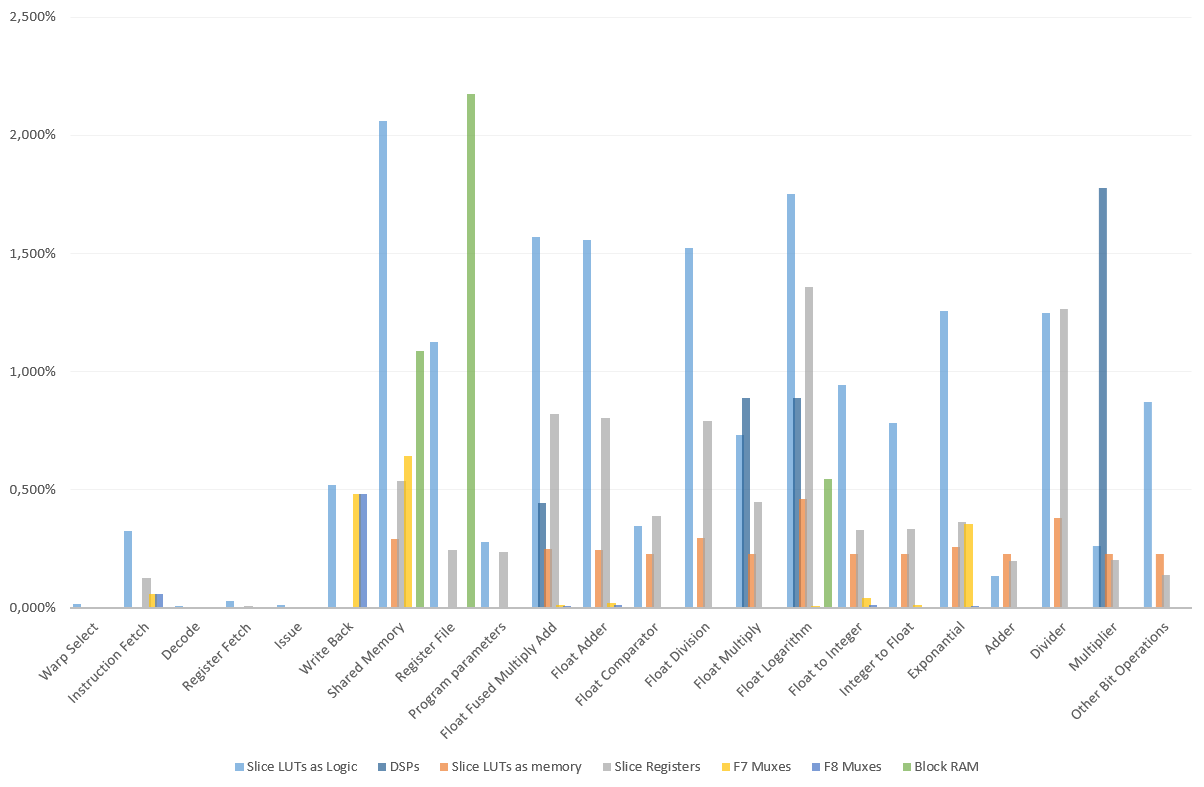
\includegraphics[width=0.9\textwidth]{gorsel/Util_S16_FMAFDIVFLOG8_FEXPDIV4.png}
\shorthandoff{=}
\caption{Ada alt modüllerinin kaynak kullanımı (Konfigurasyon 2)}
\label{image:util_S16_FMAFDIVFLOG8_FEXPDIV4}
\end{figure}

Bu konfigurasyon için float çarp-topla, float bölme ve logaritma işlemlerinde fazladan 1 çevrim, üssel fonksiyon ve tamsayı bölme işlemlerinde fazladan 2 çevrim hesap süresi; her iki gruba da fazladan 2 çevrim kuyruklama süresi eklenir. Değişiklik ile 16 adet sayının hesaplanması için harcanan süredeki değişim Tablo \ref{table:util_S16_FMAFDIVFLOG8_FEXPDIV4}'de sunulmuştur. Buradaki değişiklik, boru hattının dolması sırasında söz konusudur. Boru hattı doldurulduktan sonra "throughput" olarak her çevrimde 1 sonuç alınır.\par 

\begin{longtable}{p{90pt} p{90pt} p{90pt} p{90pt}}
\caption{Bölme, logaritma ve üssel fonksiyon hesaplama birimlerinin yarıya düşürülmesinin performansa etkisi} \label{table:util_S16_FMA16_O8} \\
\textbf{İşlem} & \textbf{Eski Hesap \newline Süresi} & \textbf{Yeni Hesap \newline Süresi} & \textbf{Yüzde Değişim} \\ 
\hline 
\endfirsthead

\multicolumn{2}{c}%
{{\bfseries \tablename\ \thetable{} -- devam}} \\
\textbf{İşlem} & \textbf{Eski Hesap \newline Süresi} & \textbf{Yeni Hesap \newline Süresi} & \textbf{Yüzde Değişim} \\ 
\hline 
\endhead

\hline \multicolumn{2}{r}{\textbf{Sonraki sayfada devam etmektedir.}} \\ 
\endfoot

\hline \hline
\endlastfoot
Float Çarp-Topla & 11 & 14 & \%27\\
Float Bölme & 12 & 15 & \%25\\
Logaritma & 14 & 17 & \%21\\
Üssel & 10 & 14 & \%40\\
Tam Sayı Bölme & 22 & 26 & \%18\\
\end{longtable}

\section{Sonuç}
ASELSAN tarafından desteklenen ve tez çalışmasını oluşturan bu yardımcı işlemci ünitesi tasarımı projesi kapsamında, temel sayısal sinyal işleme fonksiyonları için özelleştirilmiş, ölçeklenebilir ve OpenCL destekli bir paralel işlemci tasarlanmıştır. Fonksiyon listesi ve benzer mimarilerin sahip olduğu buyruk kümeleri incelenerek buyruk kümesi mimarisi oluşturulmuş, her bir buyruk için hesaplama birimleri tasarlanmıştır. Hesaplamanın paralelleştirilebilmesi için hesaplama birimleri paralel yollar üzerine kopyalanarak SIMD lane'ler oluşturulmuştur. Routing ve timing kısıtlarının sağlanabilmesi için farklı SIMD lane'ler için ortak olan işlemler tekrarlanmamıştır. Buyrukların baştan sona işlem akışı tasarlanmış ve saat sıklığının düşmemesi için boru hattı aşamalarına bölünmüştür. Boru hattının etkin kullanımı için aralıklı işleme modeli boru hattı üzerinde gerçeklenmiştir. Tasarımın ölçeklenebilirliğini artırmak ve bellek işlemlerindeki dar boğaz riskini azaltmak için hiyerarşik bir tasarıma geçilerek adalardan oluşan bir mimari tasarlanmış ve tüm yardımcı işlemci ünitesi bu şekilde gerçeklenmiştir. \par

Virtex 7 VC709 geliştirme kartı hedef platform olarak belirlenmiş, bu platforma göre devreler sentezlenerek işlem süreleri ve kaynak kullanımları ölçülmüştür.

\section{Gelecek Çalışmalar}
Proje neticesinde tasarlanan yardımcı işlemci ünitesi ölçeklenebilir ve özelleştirilebilir bir yapıdadır. OpenCL destekli olan yardımcı işlemci ünitesi için tez çalışmasının kapsamı dışında derleyici yazılmıştır. Mevcut derleyici, LLVM ara katmanını kullanarak OpenCL ile yazılan herhangi bir programı Tosun buyruklarına derleyebilmektedir. Bu noktada projenin bulunduğu noktada gerekli yazılım katmanları ile birlikte çalışabilir bir paralel işlem ünitesi vardır.\par
Gelecek çalışmaların başında en iyileme çalışmaları gelmektedir. Bellek erişimi için kaybedilen zamanın indirgenmesi ve alan kullanımında en iyilemeye gidilerek daha fazla SIMD lane gerçeklenmesi performansı dramatik şekilde artıracaktır.\par En iyileme çalışmalarının bir parçası olarak mevcut tasarım baz alınarak mimari seviyesinde yapılabilecek her bir değişim irdelenecek, bu değişimlerin performansa etkileri araştırılarak literatüre katkıda bulunulacaktır. \par
ASELSAN tarafından desteklenen Tosun işlemcisi genel amaçlı sinyal işleme algoritmaları için tasarlanmış, fakat tasarımda sağlanan standart ara yüzler sayesinde herhangi başka uygulama için hazırlanan hesaplama birimlerinin de entegre edilebileceği şekilde gerçeklenmiştir. Gelecek çalışmalarda daha spesifik uygulamalar için özel modüller entegre edilerek donanımda özelleştirme sağlanacak, böylece bir paralel hesaplama kütüphanesi kurulacaktır.  